O Shell Sort é um algoritmo de ordenação mais complexo e uma extensão do Insertion Sort. Ele começa ordenando elementos que estão distantes entre si e progressivamente reduz a distância entre os elementos a serem comparados\cite{sedgewick1986shell}. Em cada etapa, ele usa o Insertion Sort para ordenar os pares de elementos escolhidos, até que, na última etapa, a lista inteira é ordenada usando o Insertion Sort. O Shell Sort é mais eficiente em comparação com os algoritmos de ordenação simples, especialmente para listas grandes e não ordenadas, devido à sua abordagem de redução de distância.

\begin{figure}[h!]
    \centering
    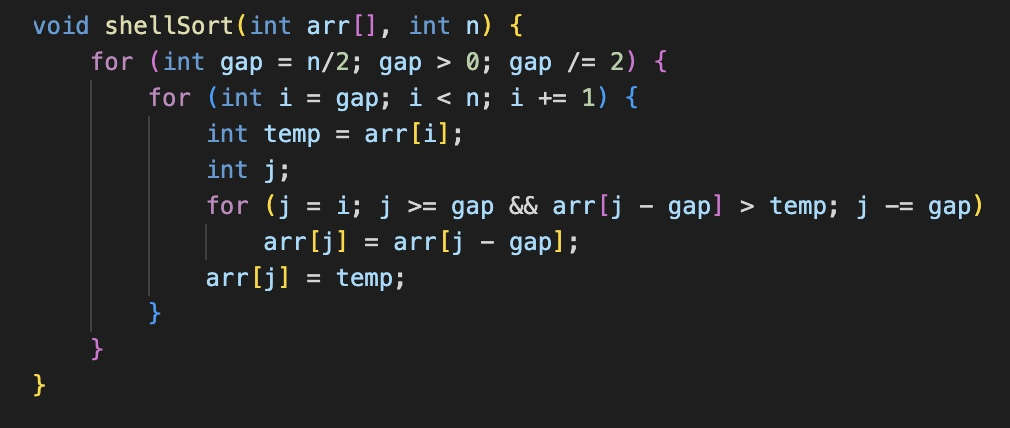
\includegraphics[width = 10cm]{Imagens/Shell Sort/ImagemShell.jpg}
    \caption{ALgoritmo Shell Sort, imagem criada pelo autor.}
    \label{fig:imagemshell}
\end{figure}

Exemplo prático Shell Sort \cite{siteShell}:
Suponha que precisamos classificar o seguinte array da figura \ref{fig:ex1}:
\begin{figure}[h!]
    \centering
    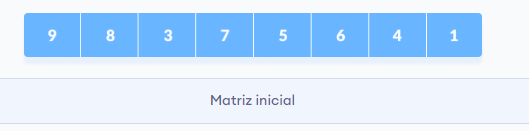
\includegraphics[width = 10cm]{Imagens/Shell Sort/ex1.png}
    \caption{Matriz Inicial}
    \label{fig:ex1}
\end{figure}

\par \newpage No primeiro loop, se o tamanho do array for N = 8 então, os elementos que estão no intervalo de N/2 = 4 são comparados e trocados se não estiverem em ordem.
O 0º elemento é comparado com o4ºelemento.
Se o 0º elemento for maior que o4ºum então, o4ºo elemento é armazenado primeiro na temp variável e o 0º elemento (ou seja, o elemento maior) é armazenado na 4º posição e o elemento armazenado tempé armazenado na 0º posição.

\begin{figure}[h!]
    \centering
    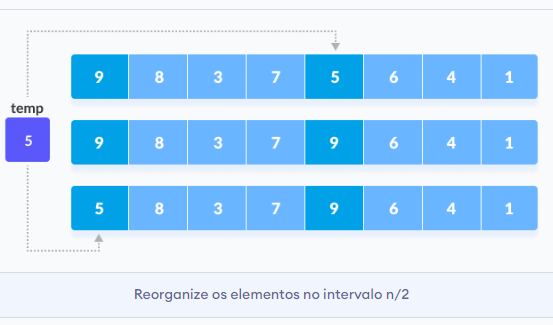
\includegraphics[width = 10cm]{Imagens/Shell Sort/ex2.png}
    \caption{Reorganize os elementos no intervalo n/2}
    \label{fig:ex2}
\end{figure}

\par Este processo continua para todos os elementos restantes.

\begin{figure}[h!]
    \centering
    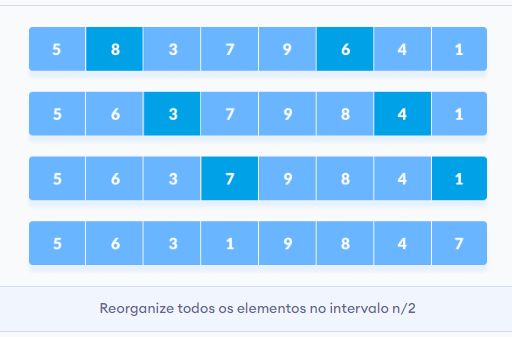
\includegraphics[width = 10cm]{Imagens/Shell Sort/ex3.png}
    \caption{Reorganize os elementos no intervalo n/2}
    \label{fig:ex3}
\end{figure}

\par No segundo loop, um intervalo de N/4 = 8/4 = 2é obtido e novamente os elementos situados nesses intervalos são classificados.

\begin{figure}[h!]
    \centering
    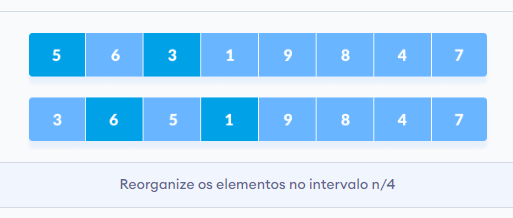
\includegraphics[width = 10cm]{Imagens/Shell Sort/ex4.png}
    \caption{Reorganize os elementos no intervalo n/4}
    \label{fig:ex4}
\end{figure}

\begin{figure}[h!]
    \centering
    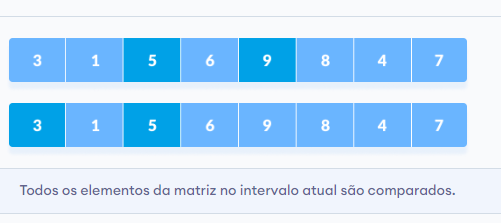
\includegraphics[width = 10cm]{Imagens/Shell Sort/ex5.png}
    \caption{Todos os elementos da matriz no intervalo atual são comparados.}
    \label{fig:ex5}
\end{figure}

\par\newpage Os elementos em 4º e 2º posição são comparadas. Os elementos em2ºe 0tha posição também são comparadas. Todos os elementos da matriz no intervalo atual são comparados. O mesmo processo continua para os elementos restantes.

\begin{figure}[h!]
    \centering
    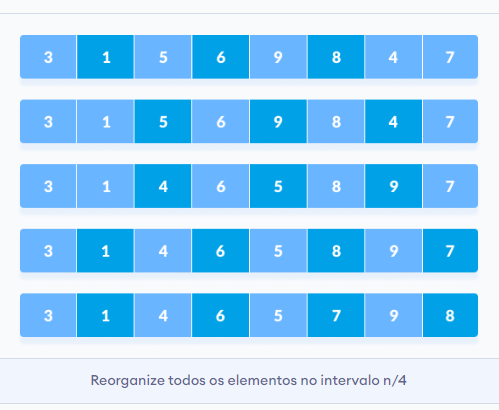
\includegraphics[width = 10cm]{Imagens/Shell Sort/ex6.png}
    \caption{Reorganize todos os elementos no intervalo n/4.}
    \label{fig:ex6}
\end{figure}

 \par E finalmente, quando o intervalo é N/8 = 8/8 =1 então, os elementos da matriz situados no intervalo de 1 são classificados. A matriz agora está completamente classificada \ref{fig:ex7}.

\begin{figure}[h!]
    \centering
    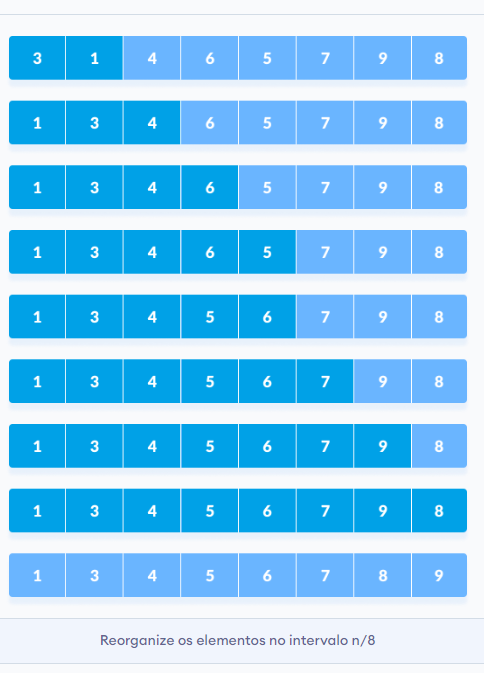
\includegraphics[width = 7cm]{Imagens/Shell Sort/ex7.png}
    \caption{Reorganize os elementos no intervalo n/8.}
    \label{fig:ex7}
\end{figure}
 

